% ---------
%  Compile with "pdflatex hw0".
% --------
%!TEX TS-program = pdflatex
%!TEX encoding = UTF-8 Unicode

\documentclass[11pt]{article}
\usepackage{amsmath}
\usepackage{amssymb}
\usepackage{jeffe,handout,graphicx}
\usepackage[utf8]{inputenc}		% Allow some non-ASCII Unicode in source

% =========================================================
%   Define common stuff for solution headers
% =========================================================
\pagenumbering{arabic}
\Class{ECE 498 ICC}
\Semester{Spring 2020}
\Authors{1}
\AuthorOne{Jin Yucheng}{yucheng9}
%\AuthorTwo{Friday Caliban}{fcaliban}
%\AuthorThree{Duncan Quagmire}{dquagmir}
%\Section{}

% =========================================================
\begin{document}

% ---------------------------------------------------------


\HomeworkHeader{1}{1}	% homework number, problem number

\begin{solution}
\item (1) There are mainly four reasons,
\begin{itemize}
\item \textbf{Parallelism}: tf.Graph explicitly shows data dependencies, making it easier for system to figure out operations that can be executed in parallel.
\item \textbf{Distributed Execution}: tf.Graph helps system to partition excution into multiple devices.
\item \textbf{Compilation}: tf.Graph can enable compiler optimization (e.g. fusion).
\item \textbf{Portability}: tf.Graph has the language-independent property, which makes it easier for users to transform models between different platforms.
\end{itemize}
\item (2) For Cloud Computing,
\begin{itemize}
\item \textbf{Advantages}: 1. Cloud Computing is a centralized design where data producers deliver data to the data centers (cloud), and data consumers request data from these data centers, which makes it easier to control and monitor data, while gives end devices remote access to the data. 2. Cloud Computing is capable of storing a huge amount of data, and enables global collaboration via networks.
\item \textbf{Disadvantages}: 1. Sending all data to cloud is not efficient, since data redundancy, bandwidth occupation, and slow response time could all significantly influence the performance of Cloud Computing. 2. Data often need some changes from producers to consumers (for example, for Youtube users, videos can be adjusted before uploading to cloud), and it requires more functions at 
the edge, which makes Cloud Computing an expensive choice.
\end{itemize}
For Edge Computing,
\begin{itemize}
\item \textbf{Advantages}: 1. Edge Computing pushes intelligence and processing capabilities to the network edge, which eliminates lag-time and saves bandwidth. 2. Connectivity, data migration, bandwidth, and latency features are pretty expensive in Cloud Computing, but in Edge Computing, data is from near sources instead of cloud, which makes it much less expensive compared to Cloud Computing.
\item \textbf{Disadvantages}: 1. Edge Computing requires higher standards for end devices, for example, end devices should have both high computational efficiency and low power consumption to give users a good experience. 2. Edge Computing requires more robust security protocols, such as strong authentication methods to proactively tackle with attacks.
\end{itemize}
\pagebreak
\item (3)
\begin{itemize}
\item Cloud Computing. Because Apple and Fitbit are big companies with a lot of users, so they need to collect a huge amount of data, and therefore Cloud Computing is preferable. Also, by uploading data to cloud, your doctor, your family can access your health data. Additionaly, Edge Computing plays a role before uploading your data to cloud, for example, the Apple watch may first perform some computations based on the data collected by sensors.
\item Edge Computing. Because the data from temperature sensors can be directly transmitted to the processing unit, and it is expensive to first upload data to cloud then access data from cloud.
\item Edge Computing. Because under this situation, less latency is important since no one wants to wait too long, and Edge Computing directly computes the data from sensors which makes the entire process faster.
\item I think the answer is both Cloud Computing and Edge Computing. Because this wearable device should send an emergency alert to local hosptials (or your families and friends), it needs to upload your data to cloud and enable other people to know your situation. Edge Computing is also required since this device should know you are falling based on computations on the data from sensors.
\end{itemize}

\end{solution}

% ---------------------------------------------------------
% Change authors for all future solutions
\AuthorOne{Jin Yucheng}{yucheng9}
%\AuthorTwo{Friday Caliban}{fcaliban}
%\AuthorThree{Duncan Quagmire}{dquagmir}
\HomeworkHeader{1}{2}
\setcounter{page}{3}
\begin{solution}
\item (1) The loss function can be rewrite as,
\begin{center}
$J(x)=
\begin{cases}
x^2& \text{$x \leq 0$}\\
0 & \text{$0 < x < 2$}\\
-x^2 + 2x & \text{$x \geq 2$}
\end{cases}$
\end{center}
the gradient of $J(x)$ is,
\begin{center}
$J^{'}(x)=
\begin{cases}
2x& \text{$x \leq 0$}\\
0 & \text{$0 < x < 2$}\\
-2x + 2 & \text{$x \geq 2$}
\end{cases}$ 
\end{center}
because the learning rate is very small, if we start from $x = -2$, since the loss function is monotonously decreasing from $-2$ to $0$, and when $x$ reaches $0$ the gradient also becomes $0$, so finally $x$ is stuck to $0$, and the value of loss function is $0$, which is a local minimum.
\item If we start from $x = 3$, since the loss function is monotonously decreasing from $3$ to $\infty$, and in theory, gradient descent brings $x$ to $\infty$ with $J(x) = -\infty$. 
\item (2) No. Because $x^2 + x + 1 = 0$ has no real roots, if we use gradient descent, the loss function will be (if the value of $J(x)$ is smaller, then $x^2 + x$ is nearer to $-1$),
\begin{center}
$J(x)= |-1 - (x^2 + x)|$
\end{center}
to minimize $J(x)$, the gradient is,
\begin{center}
$J^{'}(x)= -2x - 1$
\end{center}
which will bring $x$ to $-\frac{1}{2}$ as $J'(x) = 0$, but $x = -\frac{1}{2}$ is not a real root of $x^2 + x + 1 = 0$.
\end{solution}

% ---------------------------------------------------------
% Change authors again ; you can omit this if the authors aren’t changing.
%\AuthorOne{Hunson Abadeer}{habadeer}
%\AuthorTwo{Martin Mertens}{mmertens}
%\AuthorThree{Urgence Evergreen}{gunterno}

\HomeworkHeader{1}{3}
\setcounter{page}{4}

\begin{solution}
\item (1)
\begin{center}
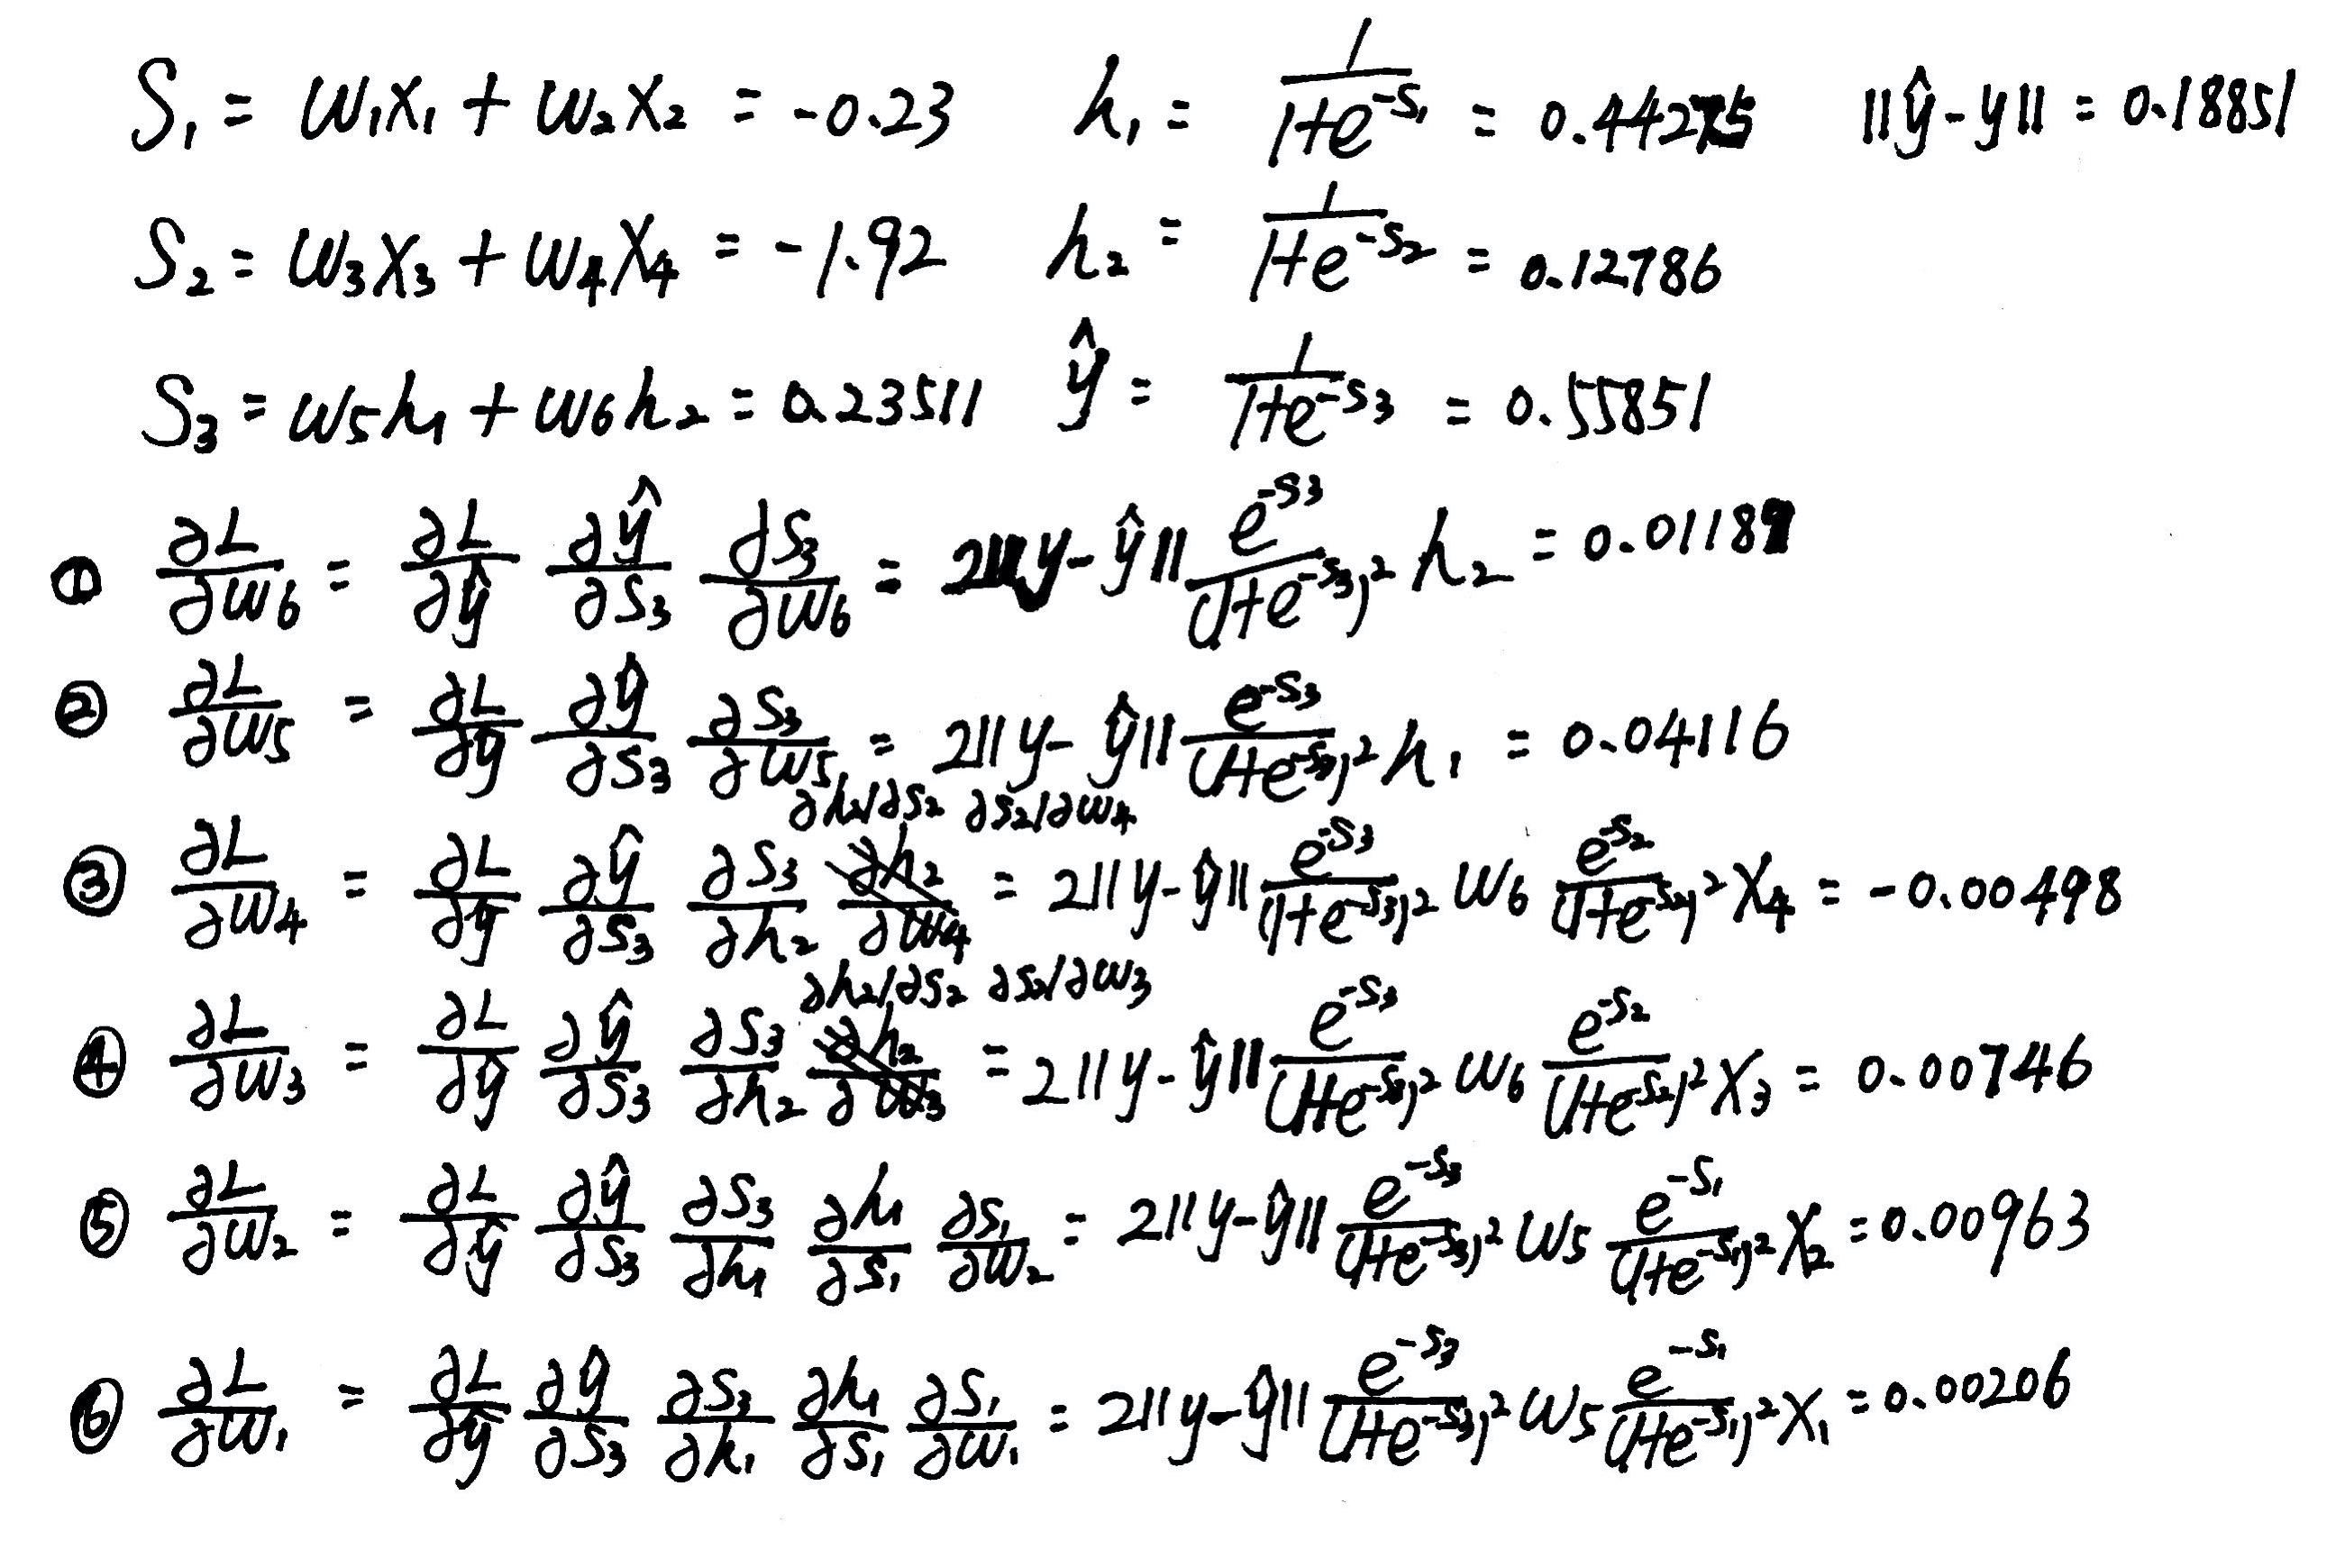
\includegraphics[width=15cm]{3.jpg}
\end{center}
\item (2) Vanishing and exploding gradients occur when training some deep neural networks,
\begin{itemize}
\item \textbf{Vanishing Gradients}: when computing gradients backward through the hidden layers, the gradients tend to be smaller in the earlier layers, since the gradients are products of terms of weights and other expressions, they may decay exponentially if the terms are less than $1$.
\item \textbf{Exploding Gradients}: is the opposite of vanishing gradients, that the gradients tend to be larger in the earlier layers, since the terms of the gradients are larger than $1$.
\end{itemize}
To solve these problems, we should initialize weights and activation functions carefully such that the products will not increase or  decay exponentially.
\end{solution}

% ---------------------------------------------------------
% Change authors again ; you can omit this if the authors aren’t changing.
%\AuthorOne{Hunson Abadeer}{habadeer}
%\AuthorTwo{Martin Mertens}{mmertens}
%\AuthorThree{Urgence Evergreen}{gunterno}

\HomeworkHeader{1}{4}
\setcounter{page}{5}

\begin{solution}
(1) Linear classifiers can learn patterns in Problem A but cannot learn patterns in Problem B. The red dots in the following figure label "0", while the black dots label "1".
\begin{center}
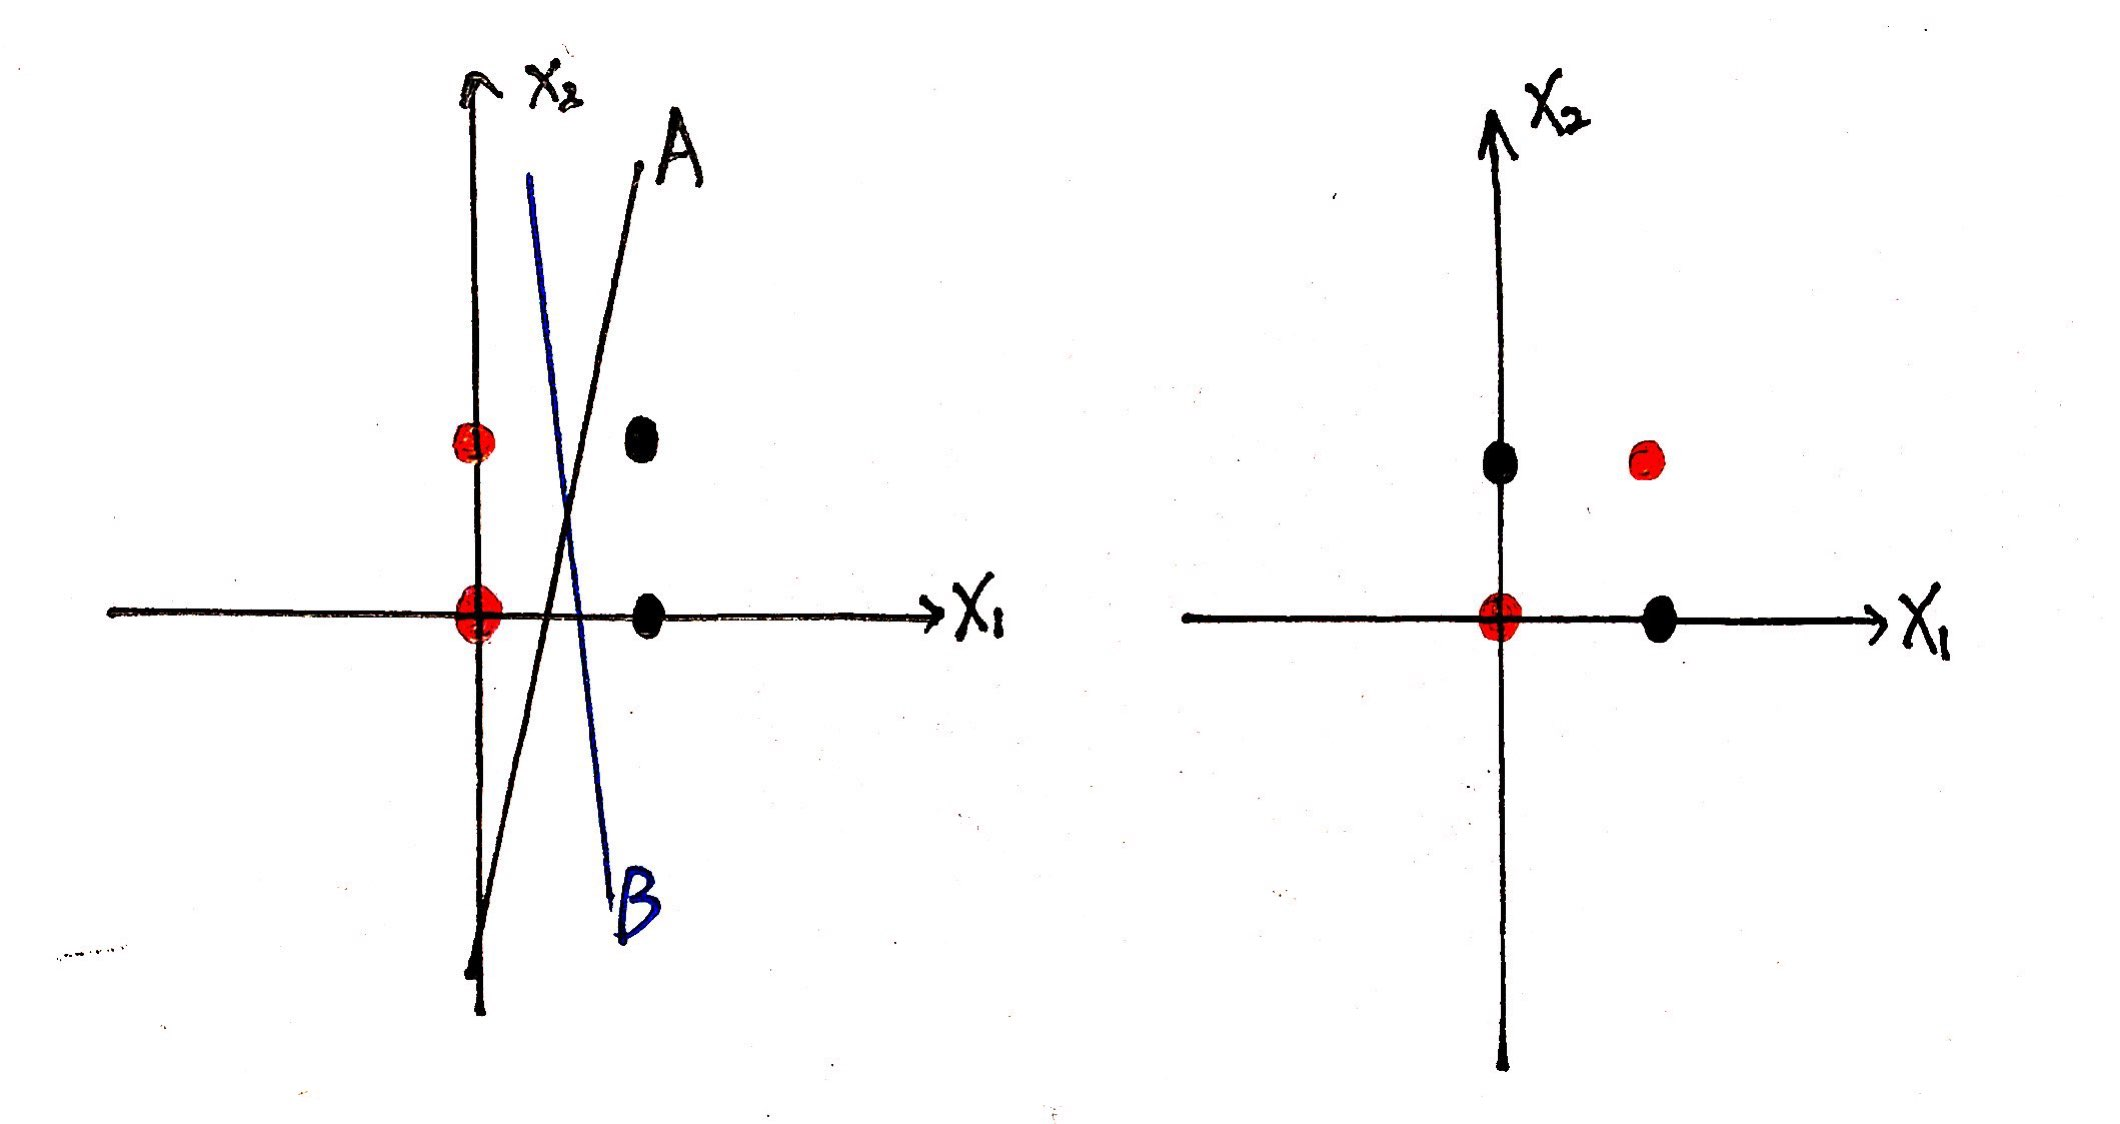
\includegraphics[width=15cm]{4.jpg}
\end{center}
For Problem A, we can see that both line A and line B can separate red and black dots (also, for example, $x_1 = 0.5$), but for Problem B, there is no such line can separate red and black dots.
\item A formal proof by contradiction,
\item \qquad Suppose there exists a line $x_2 = ax_1 +b$ that separates two categories in Problem B, then,
\item \qquad For label "0", $-b$ $(0, 0)$ and $1-a-b$ $(1, 1)$ must both be non-negative or non-positive,
\item \qquad respectively, for label "1", $1-b$ $(0, 1)$ and $-1-b$ $(1, 0)$ must both be negasitive or positive.
\item \qquad If $-b \geq 0$ and $1-a-b \geq 0$, then $1-b > 0$, which contradicts the fact that $1-b < 0$.
\item \qquad If $-b \leq 0$ and $1-a-b \leq 0$, then $-1-b < 0$, which contradicts the fact that $-1-b > 0$.
\item In conclusion, our assumption contradicts the given conditions, and dots in Problem B are not linearly separable.
\item (2) For the first neural network,
\begin{itemize}
\item The number of neurons: $16 + 32 \times 8 + 16 = 288$.
\item The number of weights: $16 \times 32 + 32 \times 32 \times 7 + 32 \times 16 = 8192$.
\item The number of biases: $32 \times 8 + 16 = 272$
\end{itemize}
So the memory requirement is $288 + 8192 + 272 = 8752$.
\pagebreak
\item For the second neural network,
\begin{itemize}
\item The number of neurons: $16 + 128 \times 2 + 16 = 288$.
\item The number of weights: $16 \times 128 + 128 \times 128 + 128 \times 16 = 20480$.
\item The number of biases: $128 \times 2 + 16 = 272$
\end{itemize}
So the memory requirement is $288 + 20480 + 272 = 21040$.
\item I prefer the first one, because it requires less memory, and it is deeper, in practice, deep neural networks are usually better than shallow neural networks.
\item (3) 
\begin{itemize}
\item The accuracy of the Multilayer Perceptron will decrease a lot, since it uses linear activation functions and is sensitive to the change in input.
\item The accuracy of the CNN will decrease a little compared to Multilayer Perceptron, because CNN is capable of extracting features thus the change of their positions will not influence accuracy much.
\end{itemize}
\item (4) Here is a comparison of ReLU, Tanh, and Unit Step Function,
\begin{center}
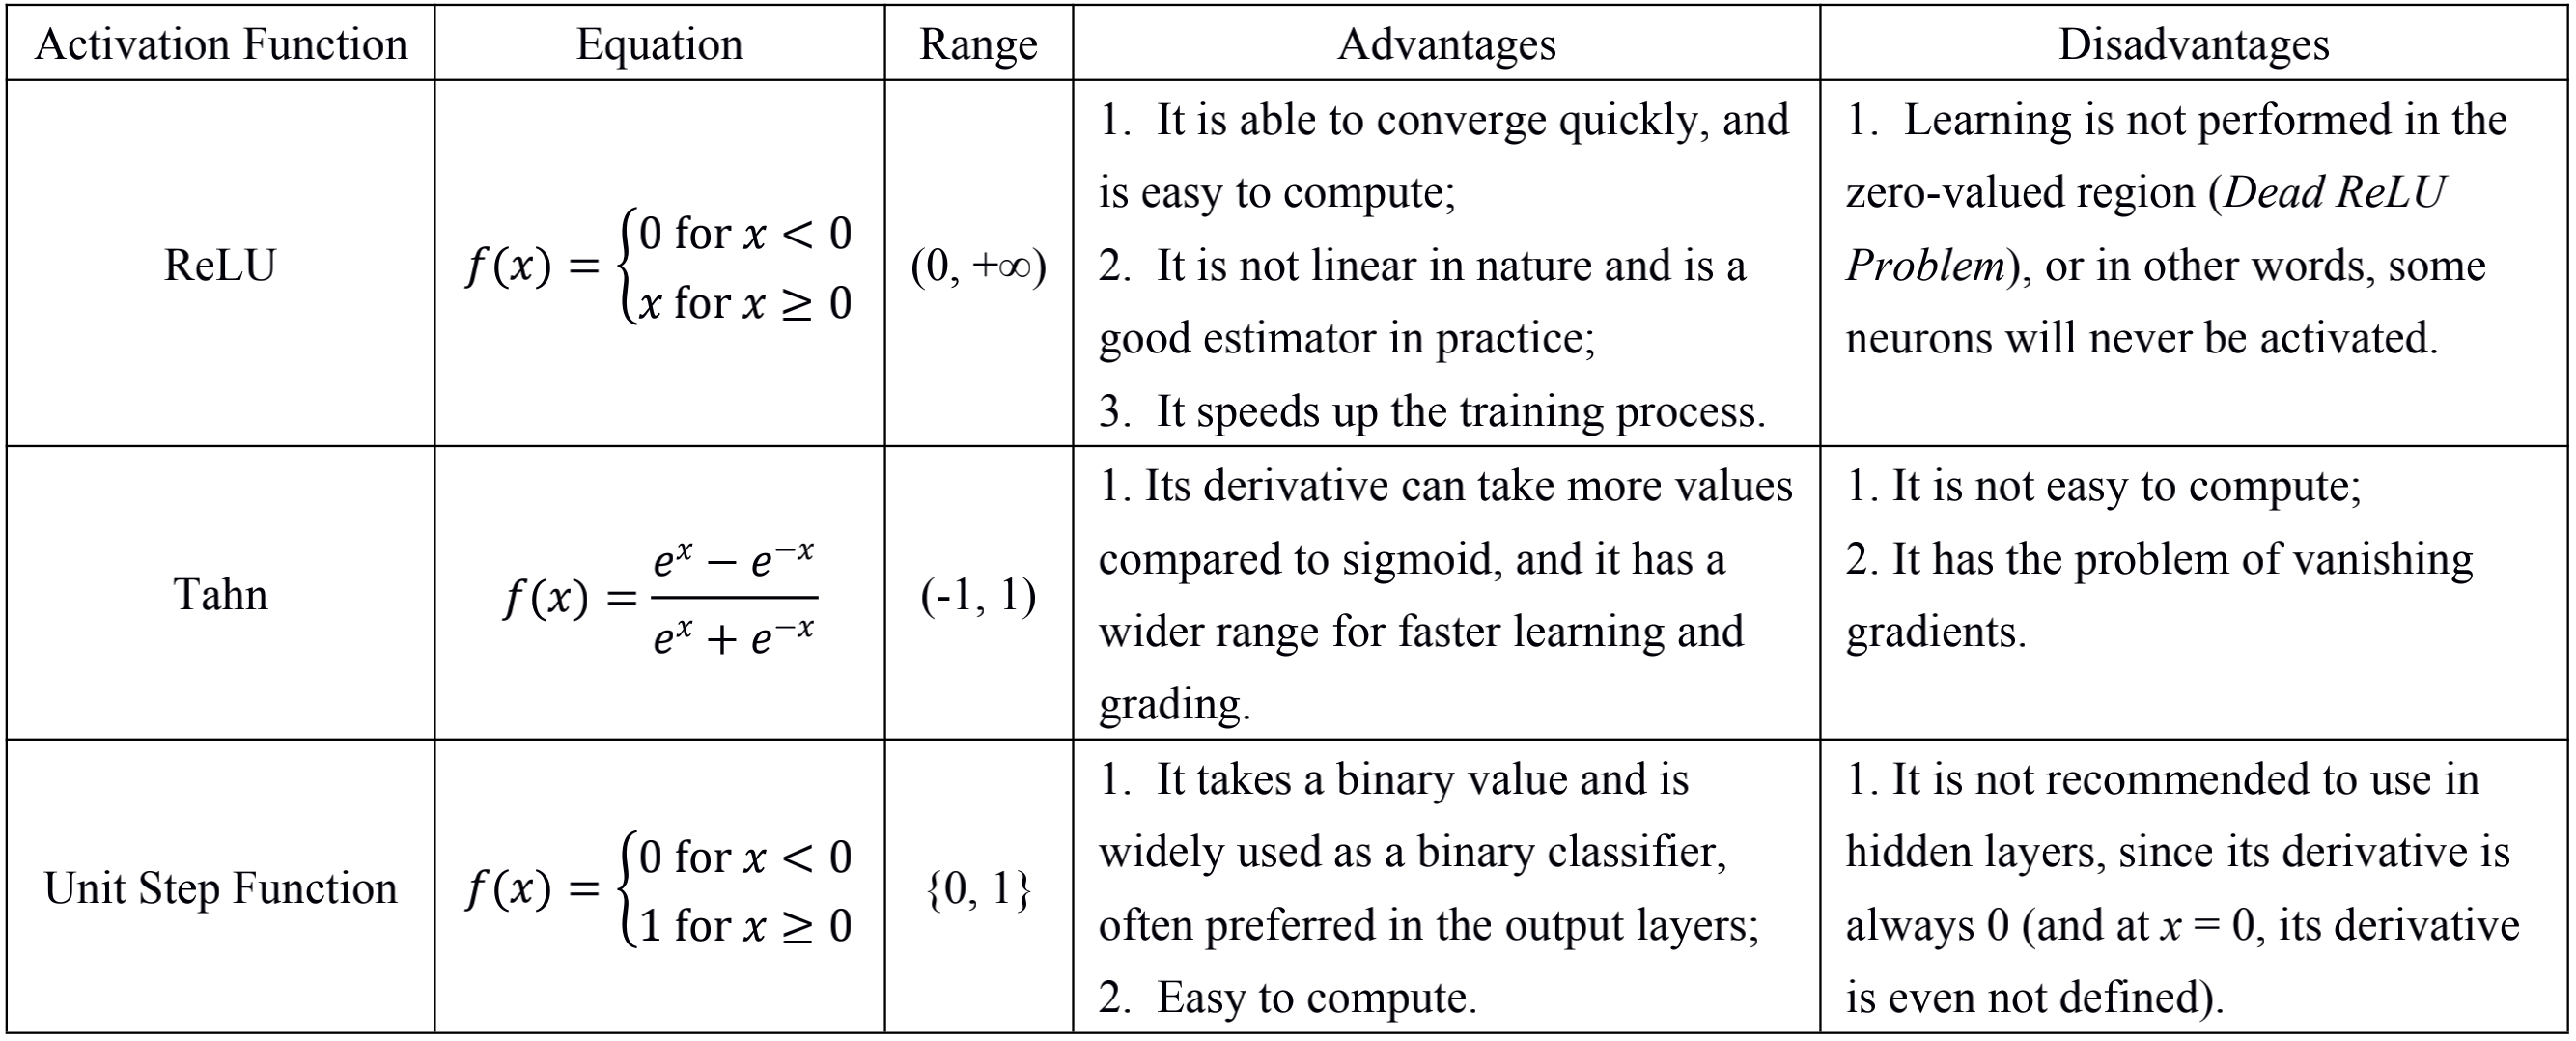
\includegraphics[width=15.5cm]{5.png}
\end{center}
\item (5) Yes. The most important disadvantage is that because classification problem deals with discrete labels, but regression problem deals with continuous labels, the conversion between continuous and discrete variables is difficult to accomplish.
\end{solution}

% ---------------------------------------------------------
% Change authors again ; you can omit this if the authors aren’t changing.
%\AuthorOne{Hunson Abadeer}{habadeer}
%\AuthorTwo{Martin Mertens}{mmertens}
%\AuthorThree{Urgence Evergreen}{gunterno}

\HomeworkHeader{1}{5}
\setcounter{page}{7}

\begin{solution}

\item (1) For matrices $A$, $B$, and $C \in R^{2^n\times2^n}$, such that $C = AB$, in the naive algorithm,
\begin{center}
$C_{ij} = \Sigma_{k = 1}^{k = 2^n} A_{ik} B_{kj}$
\end{center}
which is equivalent to, 
\begin{center}
$C_{ij} = A_{i} B_{j}$
\end{center}
where $A_{i}$ is a row vector, representing the $i^{th}$ row of $A$, 
\[ A_{i} = 
\begin{bmatrix}
    A_{i1} & A_{i2} & \dots  & A_{i2^n} \\
\end{bmatrix}
\]
$B_{j}$ is a column vector, representing the $j^{th}$ column of $B$, 
\[ B_{j} = 
\begin{bmatrix}
    B_{1j}  \\
\\
 B_{2j} \\
\\
 \vdots  \\
\\
 B_{2^nj} 
\end{bmatrix}
\]
\item (2) The naive algorithm: $112$ ($64$ multiplications + $48$ additions), Strassen's algorithm: $214$ ($49$ multiplications + $165$ additions) if optimized, $247$ ($49$ multiplications + $198$ additions) if not optimized.
\item If $A$, $B$, and $C \in R^{4\times4}$, there are totally $16$ elements in $A$, $B$, and $C$. For the naive algorithm, for one element $C_{ij}$, since $C_{ij} = \Sigma_{k = 1}^{k = 2^n} A_{ik} B_{kj}$, it takes $4$ multiplications ($2^n, n = 2$) and $3$ addition ($\Sigma$). Therefore, the naive algorithm takes $(4+3) \times 4 \times 4 = 112$ multiplications and additions.
\item The original algorithm discovered by V. Strassen in 1969 requires $7$ multiplications and $18$ additions and subtractions to compute $C \in R^{2\times2}$, but later, the number of additions and subtractions was reduced to $15$ \footnote{UTSA, CS 3343/3341: Analysis of Algorithms. "Strassen's Method for Multiplying Matices". Web. <http://www.cs-\\
.utsa.edu/~wagner/CS3343/strassen/strassen.html>. Accessed March 24, 2020.}, and the number of multiplications and additions has the following recurrence,
\begin{center}
$S(1) = 1$, $S(n) = 7S(n/2) + 15(n/2)^2$, for $n>1$ and $n$ is a power of $2$
\end{center}
for $n = 4$, $S(4) = 7S(2) + 15(4/2)^2 = 7 \times (7+15) + 15 \times 4 = 214$.
\item Among $214$ operations, $49$ are multiplications, since if we can multiply $2$ by $2$ matrices using only $7$ multiplications, then as for multiplying $4$ by $4$ matrices, we can use $7$ multiplications of $2$ by $2$ matrices, and for each $2$ by $2$ matrices multiplication, we need $7$ multiplications of numbers, so totally $49$ multiplications. Further, we can find that for matrices of dimension $2^n\times2^n$, Strassen's algorithm takes $7^n$ multiplications.
\pagebreak
\item For the original version of Strassen's algorithm, it takes $6 \times (7^n-4^n)$ additions, because at level $2^n$ there will be $18$ additions each of $2^{2n-2}$ matrix elements; at the next level, there will $\frac{7}{4}$ as many sums: the $7$ comes from there being $7$ times as many matrix products that we have to perform, the $4$ comes from the fact that they each have half the size and hence a quarter as many elements. So the number of additions is $18 \times 2^{2n-2} \times (1+ \frac{7}{4} + (\frac{7}{4})^2 + … + (\frac{7}{4})^{n-1})$, which works out to be $6 \times (7^n-4^n)$\footnote{MIT Math. "25. Strassen’s Fast Multiplication of Matrices Algorithm, and Spreadsheet Matrix Multiplications". Web. <http://www-math.mit.edu/~djk/18.310/18.310F04/Matrix\_\%20Multiplication.html>. Accessed March 24, 2020.}.
\item (3) For the naive algorithm, it takes $2^n \times 2^n \times 2^n + 2^n \times 2^n$ multiplications and additions, the asymptotic complexity is $\Theta(N^3)$, for $N = 2^n$. For Strassen's algorithm, according to the recurrence, for $N = 2^n$, its time complexity is  $O([7+o(1)]^n)$ = $O(N^{log_{2}7+o(1)})$ $\approx$ $O(N^{2.8074})$ \footnote{"Strassen's Algorithm". \textit{wikipedia.org}. Web. <https://en.wikipedia.org/wiki/Strassen\_algorithm>. Accessed March 24, 2020.}.
\item So in theory, because Strassen's algorithm reduces the number of multiplications, it is faster for calculations of large matrices than the naive algorithm. However, the reduction in the number of arithmetic operations also costs numerical stability, and requires significantly more memory compared to the naive algorithm.
\item (4) Strassen's algorithm computes $M_1$ to $M_7$ as,
\begin{align*}
M_1 &= (A_{11} + A_{22})(B_{11} + B_{22})\\ 
M_2 &= (A_{21} + A_{22})B_{11}\\
M_3 &= A_{11}(B_{12} - B_{22})\\ 
M_4 &= A_{22}(B_{21} - B_{11})\\ 
M_5 &= (A_{11} + A_{12})B_{22}\\
M_6 &= (A_{21} - A_{11})(B_{11} + B_{12})\\ 
M_7 &= (A_{12} - A_{22})(B_{21} + B_{22})
\end{align*}
and computes $C_{ij}$ as,
\begin{align*}
C_{11} &= M_1 + M_4 - M_5 + M_7 \\ \
C_{12} &= M_3 + M_5 \\
C_{21} &= M_2 + M_4 \\
C_{22} &= M_1 - M_2 + M_3 + M_6
\end{align*}
since, 
\[ A = 
\begin{bmatrix}
    A_{11}  \\
\\
 A_{12} \\
\\
 A_{21}  \\
\\
 A_{22} 
\end{bmatrix}
\qquad
B = 
\begin{bmatrix}
    B_{11}  \\
\\
 B_{12} \\
\\
 B_{21}  \\
\\
 B_{22} 
\end{bmatrix}
\]
and $C = F \otimes ((G^T \otimes A) * (H^T \otimes B))$,
clearly,
\[
G = 
\begin{bmatrix}
  1 & 0 & 1 &0 & 1& -1& 0\\
\\
 0 & 0 & 0& 0& 1& 0& 1\\
\\
 0  & 1 & 0& 0& 0& 1& 0\\
\\
 1 & 1 & 0& 1& 0& 0& -1
\end{bmatrix}
\]
because $G^T \otimes A$ must correspond to the sum of $A_{ij}$ which appears on the left side of $M_{k}$,
\[
H = 
\begin{bmatrix}
  1 & 1 & 0 &-1 & 0& 1& 0\\
\\
 0 & 0 & 1& 0& 0& 1& 0\\
\\
 0  & 0 & 0& 1& 0& 0& 1\\
\\
 1 & 0 & -1& 0& 1& 0& 1
\end{bmatrix}
\]
because $H^T \otimes B$ must correspond to the sum of $B_{ij}$ which appears on the right side of $M_{k}$.
\item$((G^T \otimes A) * (H^T \otimes B))$ gives us a vector with 7 elements, corresponding to $M_1$ to $M_7$, then,
 \[
F = 
\begin{bmatrix}
  1 & 0 & 0 & 1 & -1& 0& 1\\
\\
 0 & 0 & 1& 0& 1& 0& 0\\
\\
 0  & 1 & 0& 1& 0& 0& 0\\
\\
 1 & -1 & 1& 0& 0& 1& 0
\end{bmatrix}
\]
because every row corresponds to the coefficients of $M_1$ to $M_7$. For example, the first row calculates $C_{11}$, and $C_{11} = M_1 + M_4 - M_5 + M_7$, so the coefficient of $M_1$ is $1$, of $M_2$ is $0$, of $M_3$ is $0$, of $M_4$ is $1$, of $M_5$ is $-1$, of $M_6$ is $0$, and of $M_7$ is $1$. 
\item Observations:
\begin{itemize}
\item Each column of $G$ encodes the coefficients of $A_{ij}$ which appear on the left side of $M_{k}$.
\item Each column of $H$ encodes the coefficients of $B_{ij}$ which appear on the right side of $M_{k}$.
\item Each row of $F$ encodes the coefficients of $M_k$ that express $C_{ij}$.
\end{itemize}
\end{solution}

% ---------------------------------------------------------
% Change authors again ; you can omit this if the authors aren’t changing.
%\AuthorOne{Hunson Abadeer}{habadeer}
%\AuthorTwo{Martin Mertens}{mmertens}
%\AuthorThree{Urgence Evergreen}{gunterno}

\HomeworkHeader{1}{6}
\setcounter{page}{10}

\begin{solution}
\item (1) The curse of dimensionality refers to "various phenomena that arise when analyzing and organizing data in high-dimensional spaces" \footnote{Deming Chen, Jinjun Xiong, V. Kindratenko. "Lecture 4: Data Analytics for IoT Basics". p. 34.}. For example, when the dimensionality increases, the availabel data may become sparse as the volume of the space explodes, and with a fixed number of training samples, the performance of the ML algorithm becomes worse if we do not apply feature selection and dimensionality reduction techniques.
\item (2) Principal Component Analysis (PCA) is a statistical procedure that "uses an orthogonal transformation to convert a set of observations of possibly correlated variables into a set of values of linearly uncorrelated variables called principal components" \footnote{"Principal Component Analysis". \textit{wikipedia.org}. Web. <https://en.wikipedia.org/wiki/Principal\_component\_analysis>. Accessed March 24, 2020.}. PCA transforms the original data into a new subspace such that the projected features are orthonormal, thus enabling us to reduce features that are highly correlated, because we can choose the first $n$ principal components such that most information is maintained. In a statistical sense, variations along the axes of these $n$ principal components are higher than variations of other projected features, and are decreasing from the $1^{st}$ principal component to the $n^{th}$ principal component.
\item (3) The input data is expressed as a $n \times d$ matrix, each feature vector $\vec{x_i}$ is of dimension d,
 \[
X = 
\begin{bmatrix}
  - \vec{x_{1}} -\\
\\
 - \vec{x_{2}} -\\
\\
 \vdots \\
\\
 - \vec{x_{n}} -
\end{bmatrix}
\]
the objective is to find a $k$-dimensional subspace that captures the most information, such that every projected feature in the $k$-dimensional subspace is orthonormal (linearly uncorrelated) to each other,
 \[
V = 
\begin{bmatrix}
  - \vec{v_{1}} - & - \vec{v_{2}} - & \dots & - \vec{v_{k}} -
\end{bmatrix}
\]
notice that in $V$, every column vector is an orthonormal basis in the new subspace.
\item The relationship between $X$ and $V$ is shown by the eigenvector decomposition,
\begin{center}
$X^T X = USU^T$
\end{center}
since the first $k$ columns of $U$ are the first $k$ principal components, which just consist $V$.
\item The Frobenius norm of a matrix $X$ is a "measure" of its length, defined as,
\begin{center}
$||X||_{F} = \sqrt{\Sigma_{ij}{X_{ij}^2}} = \sqrt{tr[X^TX]}$
\end{center}
\pagebreak
it is equal to the sum of the singular values,
\begin{center}
$||X||_{F} = \Sigma_{j=1}^{d}{s_j}$\\
\item
$s_j = \Sigma_{i=1}^{N}{(\vec{u_j} \cdot \vec{x_i})^2}$
\end{center}
Therefore, to find the most important $k$ principal components, we must maximizes the Frobenious norm of the data projected onto $V$,  
\begin{center}
$\hat{V}_{pca} = argmax_{V} || X V ||_F^{2}$
\end{center}
equivalently, 
\begin{center}
$\hat{V}_{pca} = argmin_{V} || X - XVV^T ||_F^{2}$
\end{center}
such that $V^TV = I$. 
\item This objective function says that the principal components define an orthonormal basis such that the distance between the original data and the data projected onto that subspace is minimal\footnote{Jonathan Pillow. "Statistical Modeling and Analysis of Neural Data (NEU 560)". Princeton University. Web. <http://pillowlab.princeton.edu/teaching/statneuro2018/slides/notes05\_PCA2.pdf>. Accessed March 25, 2020.}.
\item Notice that it is uncommon to do PCA on uncentered data, the standard procedure is to first zero-center $X$, which means replacing each $\vec{x_i}$ with $\vec{x_i} - \overline{x}$, $\overline{x} = \frac{1}{N} \Sigma{\vec{x_i}}$. 
\item (4) Here is the proof that $\hat{V}_{pca} = argmax_{V} || X V ||_F^{2}$ and $\hat{V}_{pca} = argmin_{V} || X - XVV^T ||_F^{2}$ are equivalent,
\begin{align*}
	|| X - XVV^T ||_F^{2}
	& = tr((X - XVV^T)^T(X - XVV^T)) & \text{because ${||A||_{F}^2 = tr(A^TA)}$}  \\
	& = tr((X - XVV^T)(X - XVV^T)^T) & \text{because ${tr(A^TA) = tr(AA^T)}$} \\
	& = tr((X - XVV^T)(X^T - VV^TX^T)) \\
	& = tr(XX^T - XVV^TX^T - XVV^TX^T + XVV^TVV^TX^T) \\
	& = tr(XX^T - XVV^TX^T - XVV^TX^T + XVV^TX^T) & \text{because $V^TV = I$}\\
	& = tr(XX^T - XVV^TX^T)\\
	& = tr(XX^T) - tr(XVV^TX^T) & \text{because ${tr(A+B) = tr(A)+tr(B)}$}  \\
& = tr(XX^T) - || X V ||_F^{2}  
\end{align*}
Therefore, to minimize $|| X - XVV^T ||_F^{2}$ is equivalent to maximize $|| X V ||_F^{2}$.
\item (5) The eigendecomposition of $X^TX$ exists and the eigenvectors can form an orthonormal basis of the $d$-dimensional
space because $X^TX$ forms a symmetric matrix $\in R^{d\times d}$, furthermore, we already have the assumption that $X^TX = QDQ^T$.
\item Since $Q$ is orthonormal, $Q^TQ = I$ and $QQ^T = I$, $|| XV ||_F^{2}$ can be transformed as,
\begin{align*}
	|| XV ||_F^{2}
	& = tr(V^TX^TXV) \\
	& = tr((QZ)^TQDQ^TQZ)\\
& = tr(Z^TQ^TQDQ^TQZ)\\
& = tr(Z^TDZ)
\end{align*}
\end{solution}
% ---------------------------------------------------------
% Change authors again ; you can omit this if the authors aren’t changing.
%\AuthorOne{Hunson Abadeer}{habadeer}
%\AuthorTwo{Martin Mertens}{mmertens}
%\AuthorThree{Urgence Evergreen}{gunterno}

\HomeworkHeader{1}{7}
\setcounter{page}{12}

\begin{solution}
\item (1) To build a security system that is free of dead corner, we should make sure the viewing region of cameras covers all edges, therefore, for a single floor, the layout of cameras will be like, 
\begin{center}
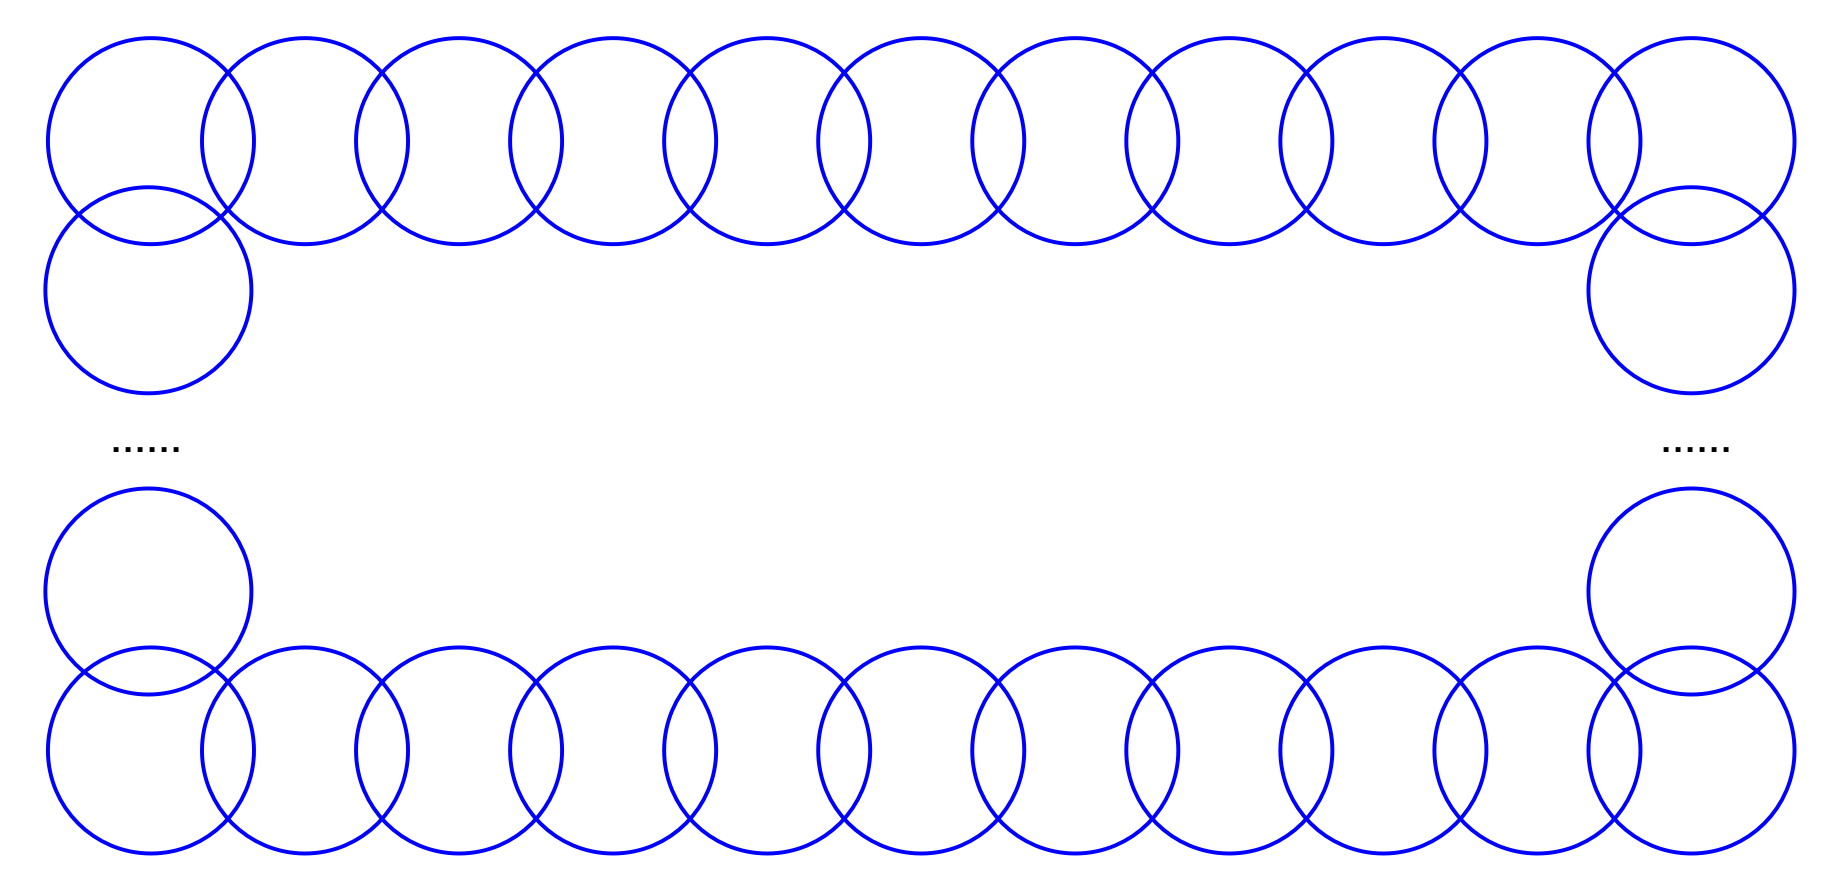
\includegraphics[width=10cm]{6.png}
\end{center}
There are $4$ cameras at $4$ corners, covering $100$ ft of the $3000$ ft edge and $100$ ft of the $2000$ ft edge respectively, more cameras are on the edges such that there is no dead corner.
\item The above configuration applies to all $3$ floors, and for each floor there is one set of IoT devices to detect intrusions, the workflow of my security system is as follows,
\begin{center}
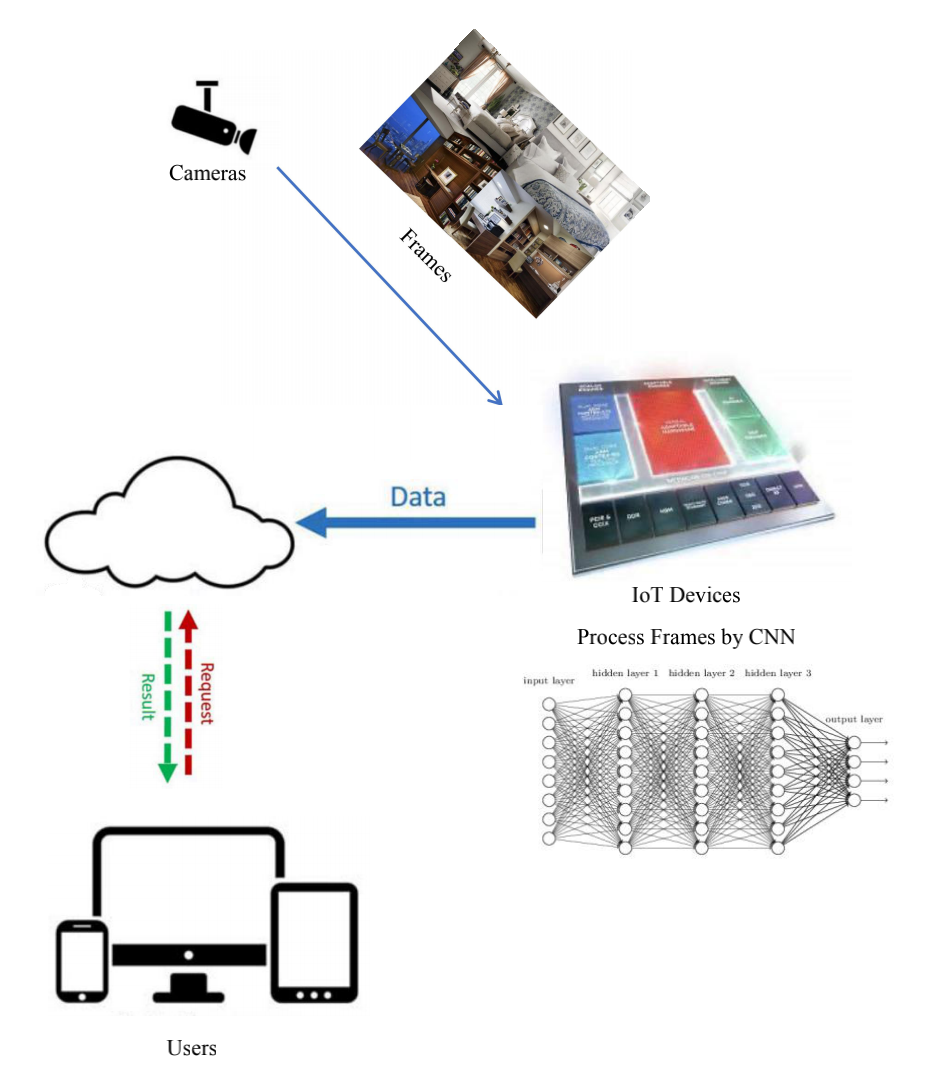
\includegraphics[width=10cm]{7.png}
\end{center}
\pagebreak
\item Frames collected by cameras are immediately passed to IoT devices, then IoT devices will use CNN to extract information from the input frames and report any result to cloud. Apps in users' devices (such as mobile phones, tablets, \& laptops) will request data from cloud regularly, and if there is intrusion, users will receive emergency alert to inform the possible intrusion.
\item (2) For one floor, there are $4 + 2 \times (2000 - 100 \times 2) / 200 + 2 \times (3000 - 100 \times 2) / 200 = 50$ cameras, so for three floors, $150$ cameras in total.
\item (3) I will choose one set of processing engines per floor, for one floor there are $50$ cameras, and each generates $10$ frames per second, so there are totally $500$ frames per second (about $1.5$ MB/s, for three floors about $4.5$ MB/s, while the bandwidth is $10$MB/s). There are several possible plans, for example, two Xilinx Cloud FPGA  (\$$4,000, 700$FPS), one Xilinx Cloud FPGA and six Nvidia Jetson TX$1$ (\$$4,100, 560$FPS), and other plans. I prefer two Xilinx Cloud FPGA, each coupled with $25$ cameras.
\item Therefore, for three floors, there will be six Xilinx Cloud FPGA (\$$12,000, 2,100$FPS), each coupled with $25$ cameras.
\item (4) $150$ cameras cost \$$1,500$, six Xilinx Cloud FPGA cost \$$12,000$, the total cost is \$$13,500$.
\item (5) First, we must look at $2$ seconds ($2,000$ milliseconds) of footage; second, as cameras capture frames, it takes about $300$ to $600$ milliseconds for Xilinx Cloud FPGA to access frames. Since one Xilinx Cloud FPGA is coupled with $25$ cameras and is able to process $350$ frames per second, it takes about $80$ to $200$ milliseconds for Xilinx Cloud FPGA to process frames. Therefore, the average worst-case latency for detecting an intrusion is about $2,400$ to $2,800$ milliseconds.
\item \textit{Above is the discussion under the assumption that only covering edges is enough. If we want to fill in the whole area, then we need,}
\item (2) For one floor, there are $3000 \times 2000 / (200 / \sqrt{2})^2 = 300$ cameras, so for three floors, $900$ cameras in total. This may not be the optimal solution, but according to the figure below, if we cover the entire area with the orange inscribed squares within the viewing region, then we can ensure that there is no dead corner left.
\begin{center}
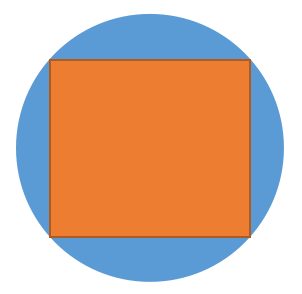
\includegraphics[width=2.5cm]{8.png}
\end{center}
\item (3) For one floor, there are $300$ cameras, and each generates $10$ frames per second, so there are totally $3000$ frames per second, we need $8$ Xilinx Cloud FPGA (\$$16,000, 2,800$FPS) and $10$ Xilinx PYNQ Z$1$ (\$$2,000, 200$FPS). Each Xilinx Cloud FPGA is coupled with $35$ cameras and each Xilinx PYNQ Z$1$ is coupled with $2$ cameras.
\item Therefore, for three floors, there will be $24$ Xilinx Cloud FPGA and $30$ Xilinx PYNQ Z$1$, each Xilinx Cloud FPGA is coupled with $35$ cameras and each Xilinx PYNQ Z$1$ is coupled with $2$ cameras.
\item (4) $900$ cameras cost \$$9,000$, $24$ Xilinx Cloud FPGA cost \$$48,000$, $30$ Xilinx PYNQ Z$1$ cost \$$6,000$, the total cost is \$$63,000$.
\item (5) Because each Xilinx Cloud FPGA and each Xilinx PYNQ Z$1$ are computing in full capacity, now it takes about $450$ to $900$ milliseconds for them to access frames, and about $100$ to $240$ milliseconds for them to process frames. Therefore, the average worst-case latency for detecting an intrusion is about $2,600$ to $3,200$ milliseconds.

\end{solution}

\end{document}
